\hoofdstuk{Defining native}
\paragraaf{Introduction}
This chapter will define the paradigm of \emph{native look-and-feel}.

\paragraaf{Native mobile applications}
A native application is an application inherent to the platform for which it was built using techniques proprietary to the platform. For example, an iOS application is native when written in Objective-C and an Android application is written in Java. Native applications are typically fast and can access the device's native API's.

\subparagraaf{The native look-and-feel}
When written in the native framework for a platform a mobile application receives acces to the available public libraries of the platform. These libraries include the UIKit\emph{(on iOS)} which provides the developer with a pre-fabricated set of user interface components. These can be seen as the building blocks for the graphical user interface on that platform. When used, the general style of the mobile application gains consitency to the overal user interface design of the platforms operating system. This gives an application its native look, which in turn participates to the \emph{native feel}.

%with a feeling of recognition when using the application, userinterface elements work as they expected based upon experience with using the operating system.
%todo: add some notes about the Human Interface Guidelines.

The \emph{native feel} of a mobile application can be defined as the speed in which the userinterface elements, the responsiveness of user interface elements to touch events, and smoothness of the animation in which the user interface elements are moved. A native mobile application has the advantage to hardware acceleration. This means its code has been precompiled and directly executed by the device CPU, rather than having to be interpreted by the device's browser. As a result of this the user interface elements are rendered faster and it \emph{feels} smooth.
 	

\paragraaf{Alternative mobile application types}
\subparagraaf{Web applications}
A mobile web application is an application developed with web technologies as JavaScript and HTML5 with CSS3. It is in fact nothing more than a website designed to fit on mobile devices, often they resemble the style of a native application rather than a traditional website. These applications are build with a JavaScript library to add support for scrolling and handling touch events. Touch events are handled via user interface elements provided by the library. Examples of these libraries include jQtouch, SenchaTouch.

% todo: screenshots/links neerzetten.

\subparagraaf{Hybrid applications}
A hybrid application in mobile development refers to an application which use a native shell to wrapped around web app. There are generally two forms of native shells, the first is a \emph{webview} and the second a native framework which exposes a javascript API to provide the web application access to otherwise native API's.

\subparagraaf{Webview-based hybrid applications}
A webview-based hybrid application is a webbased mobile application wrapped in a webview. A webview is a view or element which acts like a browser would, e.g. it is able to render HTML and run javascript.  It is readily available in the native libraries. The advantage of a webview-based hybrid application over an normal web application is that it can be published via the devices native application publishing platforms. e.g. a webview-based hybrid application targetted for the iPhone can be placed in the Apple appstore. 

Worklight is an example of a framework which can be used to develop webviewbased hybrid applications.

\subparagraaf{Framework hybrid applications}
A Framework based hybrid application is a webviewbased application build upon a framework which provides an API to allow the application access to otherwise native API's. The framework is written in the platforms native programming language making it possible to access the native API, such as reading contact list, composing of SMSes, full access to the location API, etc.

PhoneGap is an example of a framework which can be used to develop mixed hybrid applications.

\paragraaf{Comparison}
Web applications are quick and cheap to develop. Written entirely in HTML5, CSS and JavaScript. Executed by the mobile
browser and therefore cross - platform by default, but less powerful than native apps.
 
Hybrid Applications (Web), the app's source code consists of web code executed within a native wrapper that is provided by a framework.
 
Hybrid Applications (Mix), the developer augments the web code with a Javascript API to create unique features and
access native APIs that are not yet available via the browser, such as AR, NFC and others.
 
Native Application are platform-specific. Requires unique expertise and knowledge. Pricey and time consuming to develop but
 delivers the highest user experience of all approaches.

\begin{centering}
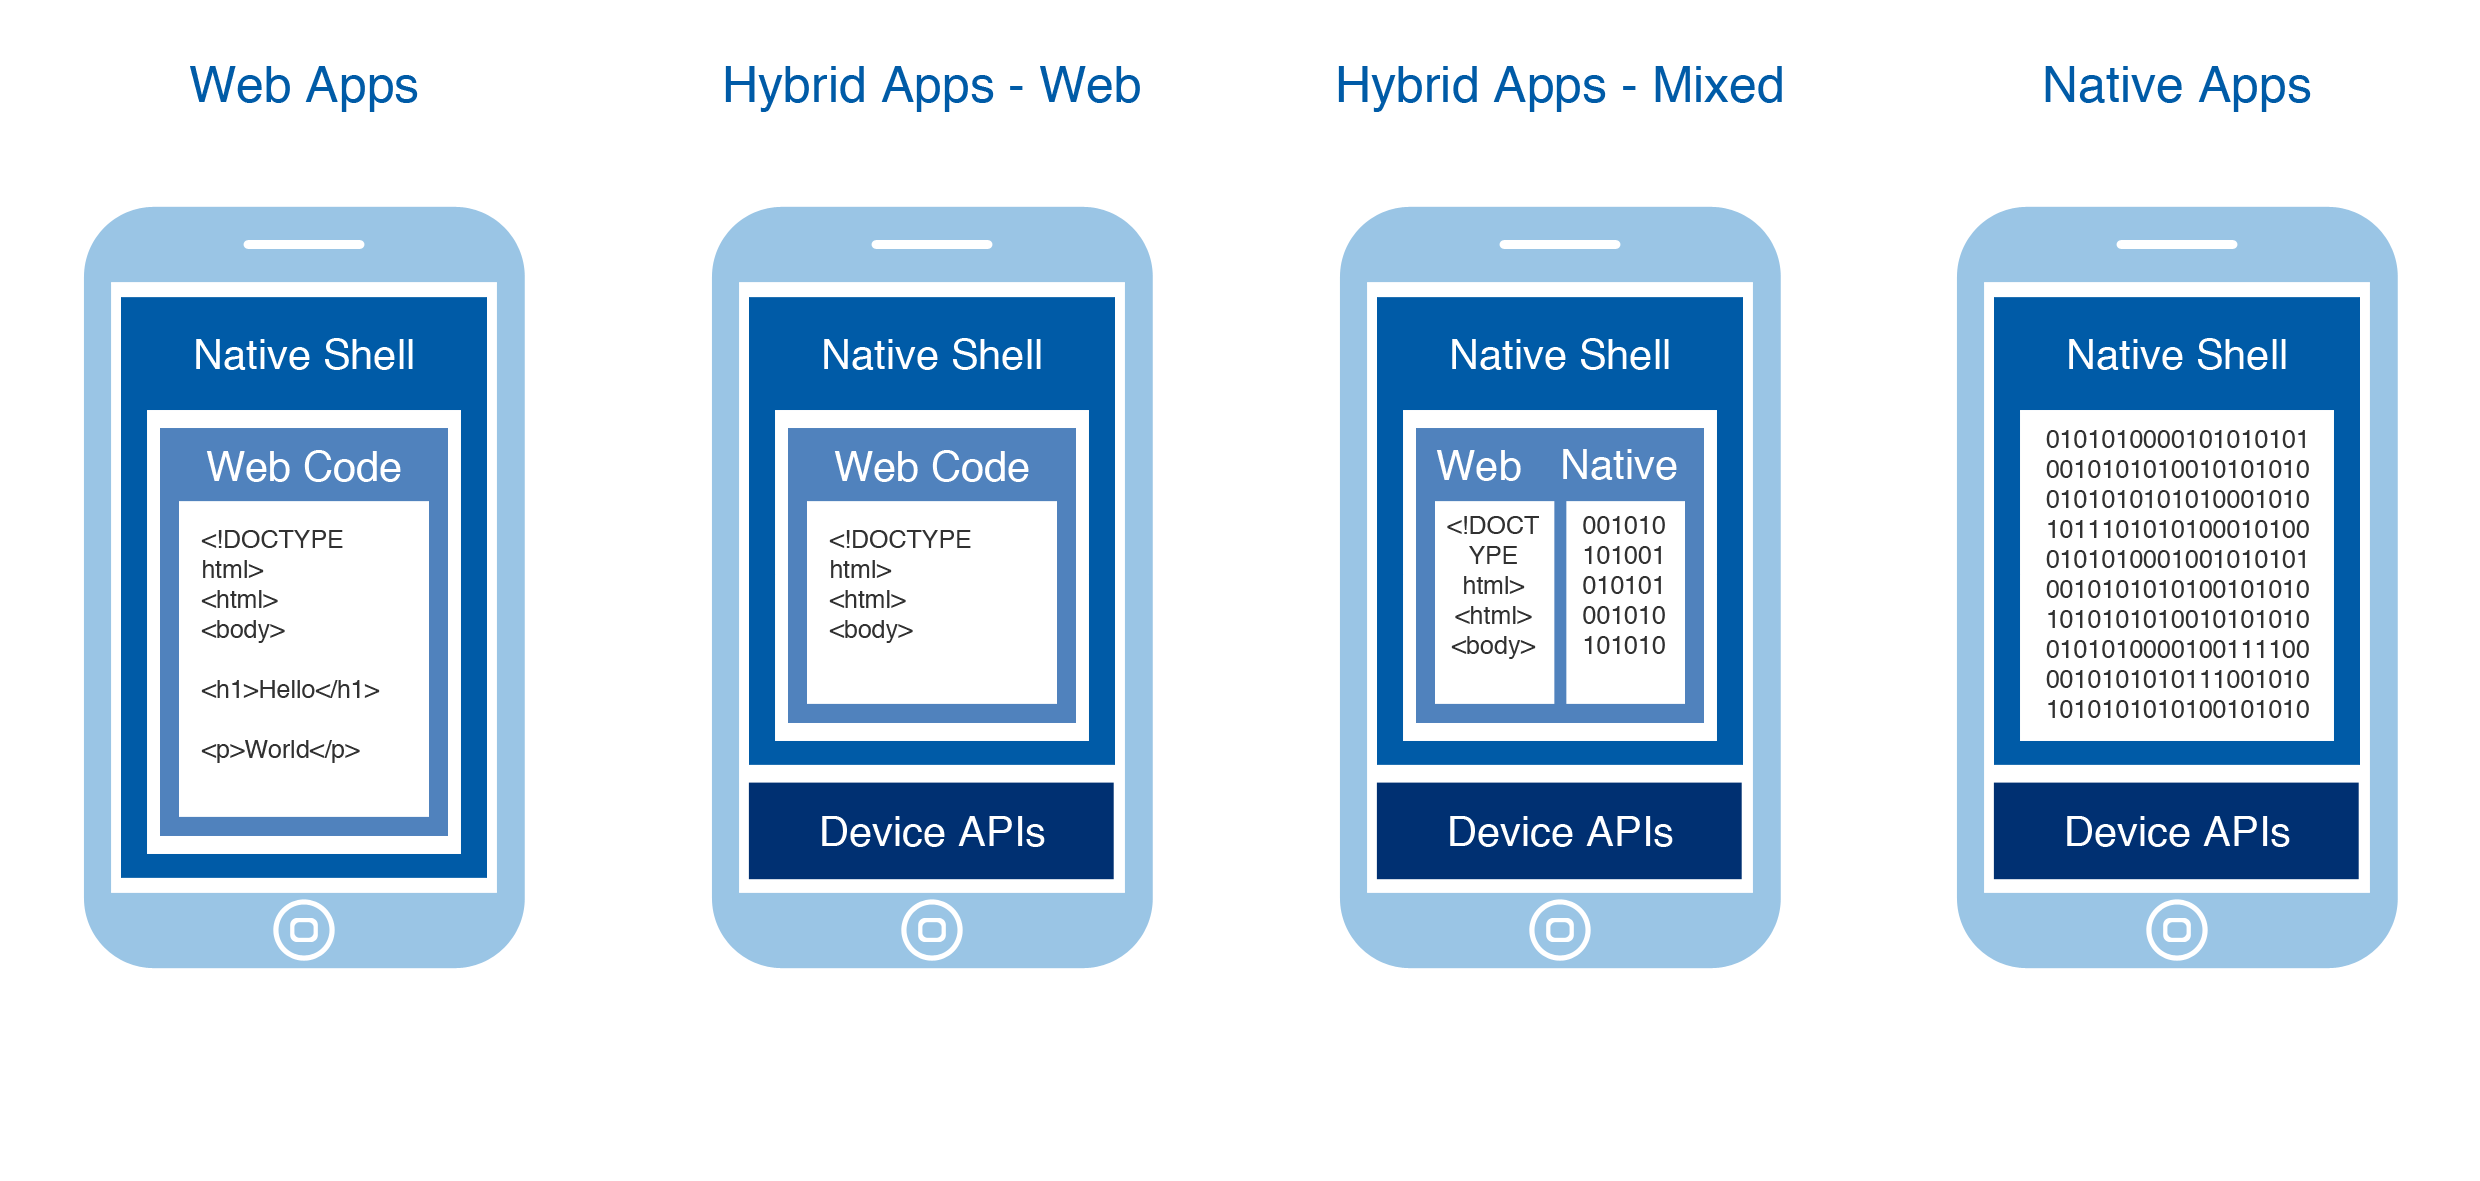
\includegraphics[scale=0.5]{images/apptypesdefined.png}\\{Different types of mobile applications\cite{IBM-Worklight2012}}\\
\end{centering}

\paragraaf{Conclusion}
A nativily written mobile application provides the user with an experience immersed to that of the level of the device's operationg system. This is due to two reasons:
\begin{itemize}
\item
\emph{Performance}\\
a native application is faster because it has direct access to memory and CPU
\item \emph{Looks}\\
a native application looks and feels more coherent to the device's operatingsystem because it is able to make use the of the provided userinterface elements.
\end{itemize}


